%% This is an example first chapter.  You should put chapter/appendix that you
%% write into a separate file, and add a line \include{yourfilename} to
%% main.tex, where `yourfilename.tex' is the name of the chapter/appendix file.
%% You can process specific files by typing their names in at the 
%% \files=
%% prompt when you run the file main.tex through LaTeX.
\newcommand{\repeatcaption}[2]{%
  \renewcommand{\thefigure}{\ref{#1}}%
  \captionsetup{list=no}%
  \caption{#2 (repeated from page \pageref{#1})}%
}

\chapter{4. Design and Implementation}

\section{Case Study: bikebump}
To test a system of that handles data collection through plan
prioritization, an application for improving bike lanes was selected for a
case study. Using bikes for commute has been a trend through recent years
though the U.S., one consensus shows that there was a 3\% increase of
people choosing bikes for everyday transportation from 2010 to 2013 and is
close to double compared to the year 2000.\cite{debra2016onemillion} We can see the trend of cities investing on improving bike lanes are in sync especially in dense city areas. New York city has had 400 miles of cycle path renewals starting from the 2000s. The field of public health public health supports this by research by showing investment on bike lanes are efficient compared to other public health interventions.

\subsection{Urban Planning}
Urban planning interventions tend to have exceptional cost impact, yet the process for deciding which to execute is also long and tedious. Because of this slow process and cost impact, it is difficult to make the proposal creation as a learning process. 
In the united states, the construction cost for a highway is 8million to 10 million USD per mile, where one of the most expensive bike lanes will cost 445,000 USD per mile. Bike lanes relatively inexpensive, starting with simply paint. Moreover these interventions are reversible, which enables to iterate for try and error.

It is certain that like painting bike lanes are cheap reversible thus may be able to make the process fast, but some interventions are expensive and requires lots of domain knowledge and engineering which inevitably will be a slow process. It is difficult to design or even reach a consensus within the community, because of the duration, a tentative pole may not directly reflect the demand of citizen when the construction is actually completed, especially where people tends to move frequently. Yet there are examples that the demand of such long and costly infrastructure is decreasing, since this relates to different types of transportation people uses. If the trend of the number of cars decrease continues and multi modal transportation is accepted, light interventions such as bike lane improvements will raise the share, supported by the trend of the increase of population density, the cost impact per population will be decrease.

\section{Current Method for Changing bike related infrastructure}

The Transportation Improvement Program is a federal requirement for each state listing improvements for transportation all needs. This is the standard way though U.S. and bikeway improvements are included.

\begin{figure*}[!htb]
  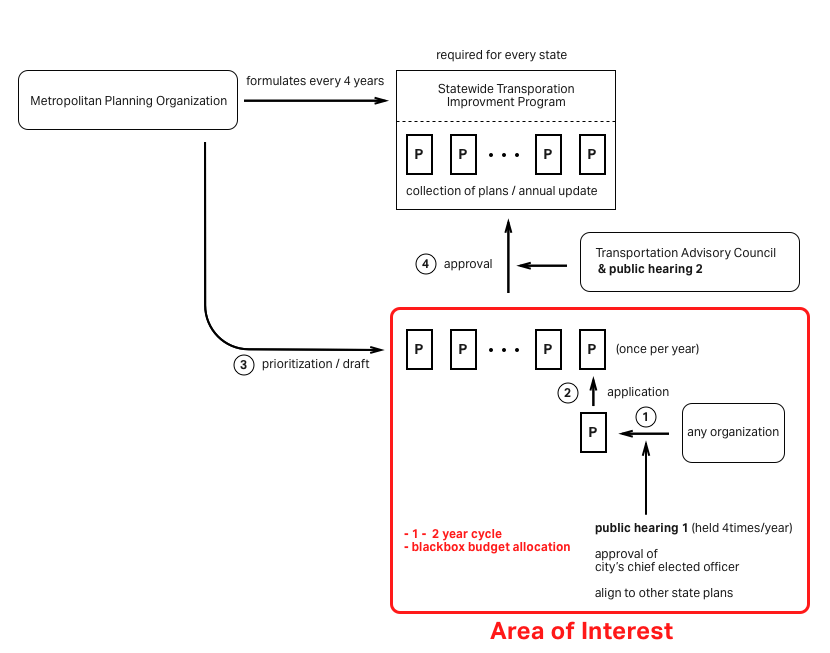
\includegraphics{chapters/4/fig/tip_process.png}               
  \caption{TIP(Transportation Improvement Program) required by each state. \url{https://www.gpo.gov/fdsys/pkg/USCODE-2011-title23/html/USCODE-2011-title23-chap1-sec135.htm} 
  }
  \label{fig:tip_process}
\end{figure*}

\begin{enumerate}
\item The process starts with a the city level required to have least one public hearing, and approval of the city's mayor. This needs to be aligned to be aligned with the state level manifesto.
\item After meeting the city level criteria, it is scrutinized by the local office of Metropolitan Planning Organization. The MPO evaluates and engineers the proposal to a executable plan. The MPO also prioritises the plans.
\item The list of plans will be undergoing a second public hearing and discussed with the Transportation Advisory Council.
\item Once approved the proposal will be listed into one plan inside the Statewide Transportation Improvement Plan.
\end{enumerate}

\begin{figure*}[!htb]
  
\includegraphics[width=\textwidth]{chapters/1/fig/proposed_process.png}               
  \repeatcaption{fig:proposed}{proposed method}
\end{figure*}

Other process such as Cambridge Participatory Budgeting project is capable of assigning budget to road infrastructure improvements. The current method provides a way to submit an idea to any given point of the city. The ideas are based on subjective comments and no cost estimation is there, with no data to support the claim.
Figure \ref{fig:proposed} shows the alternative method using bikebump. The main difference compared to the present standard procedure is; 1. Has a data collection method 2. Individual planning will be though the system, 3. City chief elected officer and the planning organization will commit by approving the system and modifying the metrics to meet with longer term goals that should be consistent to previous settlements and plans.


\clearpage

%steps for planning "community engagement"
%Determine the goals of the plan improve bike lane security
%not just reactive, but to start predicting potential threats
%Plan out who to engage
%bike advocacy groups
%Develop engagement strategies for the those individuals you already know
%bike advocacy groups
%Develop engagement strategies of those individuals you do not already know
%general community, including people using different
%Prioritize those activities
%Create an implementation plan
%Monitor your process
%Maintain those relationships

\section{Implementation Overview}

% The browser provide functionalities to record and process 
% 
% short description on the technological implementation
% web application, (client and server)
% few technologies used for bike bump
% The bikebump web application leverages various Web API's offered by browser programs
% Other libraries, but most notably React framework
% current web development are rapidly changing, javascript itself is a highly collective, programming language.
% Server
% for database, NoSQL Service based firebase offered by Google.
% [Diagram showing implementation]

This section goes through the implementation and techniques used for developing the application. The application is based on modern browsers, which recently extends the capabilities that were limited to mainly text and images. The WebRTC (Real Time Communication) is a series of protocols and APIs specifically for capturing audio and images and use them as inputs without plugins. The bike bump app leverages this technology to capture sound data. FFT will be applied to use get the frequency distribution of the called Web Audio API, 

Appendix XXX provides the extensive list of used APIs for developing the application.

The application is structured in form of a web application, which
components are the database, back end server, front end client. The database is a NoSQL, which stores data as a giant JSON data. To reduce the number of requests and efficient data transfer, the database contains some redundancy in memory.

\subsection{Definition}

The following is the definition for certain element that consist in the app.
% TODO: add image

\textbf{DING}

A DING is a spatial representation of a ring bell report. It defines the
geofence of the ding, with a center geolocation and radius. It also hold
information for each report which is the timestamp, users id and the
``good''/``bad value based on the study protocol. If there is a road near by the center location, it will also contain the roads identifier and distance from the closest point of that road.

\textbf{ROAD}

A ROAD is a geometrical feature that is returned by the Vector map API call. (Appendix. XX Vector Maps). A newly created ding will find the closest road registered in the Openstreetmap database and geometrical features will be copied to the bike bump database. When creating a improvement plan, users will first need to choose which road to apply an intervention.

\textbf{COMMUTE}

A COMMUTE is series of GPS location data, to know whole path of each ride session. Raw GPS data has tendency to bounce and contain noise, so it will be processed to match the road network in Openstreetmaps. Appendix XX shows which method was taken for getting the estimated path.

\textbf{BIKE COINS}

BIKE COINS are the currency for deciding which intervention to
prioritize. Each users will initially receive 100 BIKE COINS, which can be
distributed by the users choice.

\textbf{IMPROVEMENT PLAN}

A IMPROVEMENT PLAN is a combination of a CONTEXT and a SOLUTION.This
method of having a separate list of where (CONTEXT) and what (SOLUTION) and
combining them is taken from Christopher Alexander`s methodology of ``The
Pattern Language.''
\cite{alexander1977pattern}

The method of defining patterns (a recipe what to do in order to come up
with in outcome) and apply them to common cases is widely used in the realm
of software engineering as design patterns.
\footnote{although Alexander himself claims that ``design patterns'' in
  software is different to what he had create, since the patterns are distinctive, having no
interrelation between them.\url{https://www.youtube.com/watch?v=98LdFA-_zfA}}

Each IMPROVEMENT PLAN holds information of how many BIKE COINS it requires
to be counted as a community approved plan. This number can be calculated
using the SOLUTION`s type and unit cost, multiplied by the length of the
road.

\textbf{SOLUTION}

This is the execution instructions for a possible plan, such examples are
creating Bike Boxes and painting the lane with green paint.
This is separate from the CONTEXT focusing on only what to do for a
road, equivalent as the patterns in the Pattern Language.
Information that is included in one solution is name, description, type and
unit cost. The type is used to differentiate the solution needs to account
the length of the improvement or not. For example, a bike box will only be
needed for one intersection, where painting a lane in green will differ
with the total length. The unit cost is how much BIKE COINS would be
necessary per unit which is defined by the type. The unit cost will be
connected to the cost of the intervention. The cost will include but will
not limit to monetary cost, since some solutions will be
politically difficult even in relatively cheap interventions. 

For the experiment, three solutions where provided (Table \ref{tab:solution}).

\begin{table}
  \centering
  \begin{tabular}{|c|c|c|}
    SOLUTION & type & unit cost (m) \\ \midrule
    Green Paint & road & 25\\ 
    Bike Box & intersection & 320\\ 
    Plastinc Polls & road & 75 \\ 
  \end{tabular}
  \caption[solutions]{Solutions provided for Experiments.
    Values are estimated by material cost. Dimensions are taken from the
    Urban Bikeway Design Guide\cite{national2014urban}. Green Paint is
    \[5ft (W) * 2 (both sides)\] 
    BikeBox is
    \[12ft (W) * 16ft (H) \]

    Cost estimation can be done here 
    \url{http://www.asphaltkingdom.com/parking-lot-paint-calculator}

    Plastic polls are put in 2m pitch with each costing \$150
    \cite{aarian2016want}, therefore
    \$75 for each meter. 
  }
  \label{tab:solution}
\end{table}
\\

\textbf{CONTEXT}

The CONTEXT is a segment of a road which a Solution will be applied. The
system enables the users to select which part of a road they would like to
improve. The segment will include information of the length to by
multiplied to the unit solution cost if applicable.

% The browser provide functionalities to record and process 
%
% short description on the technological implementation
% web application, (client and server)
% few technologies used for bike bump
% The bikebump web application leverages various Web API's offered by browser programs
% Other libraries, but most notably React framework
% current web development are rapidly changing, javascript itself is a highly collective, programming language.
% Server
% for database, NoSQL Service based firebase offered by Google.
% [Diagram showing implementation].
\section{Interface}

The app has five major views; the recording view, the map view, the
vote view, the improvement list view, and improvement creation view. The
top navigation bar guides the user to jump between the views.

\subsection{Record view}

\begin{figure}[!htb]
  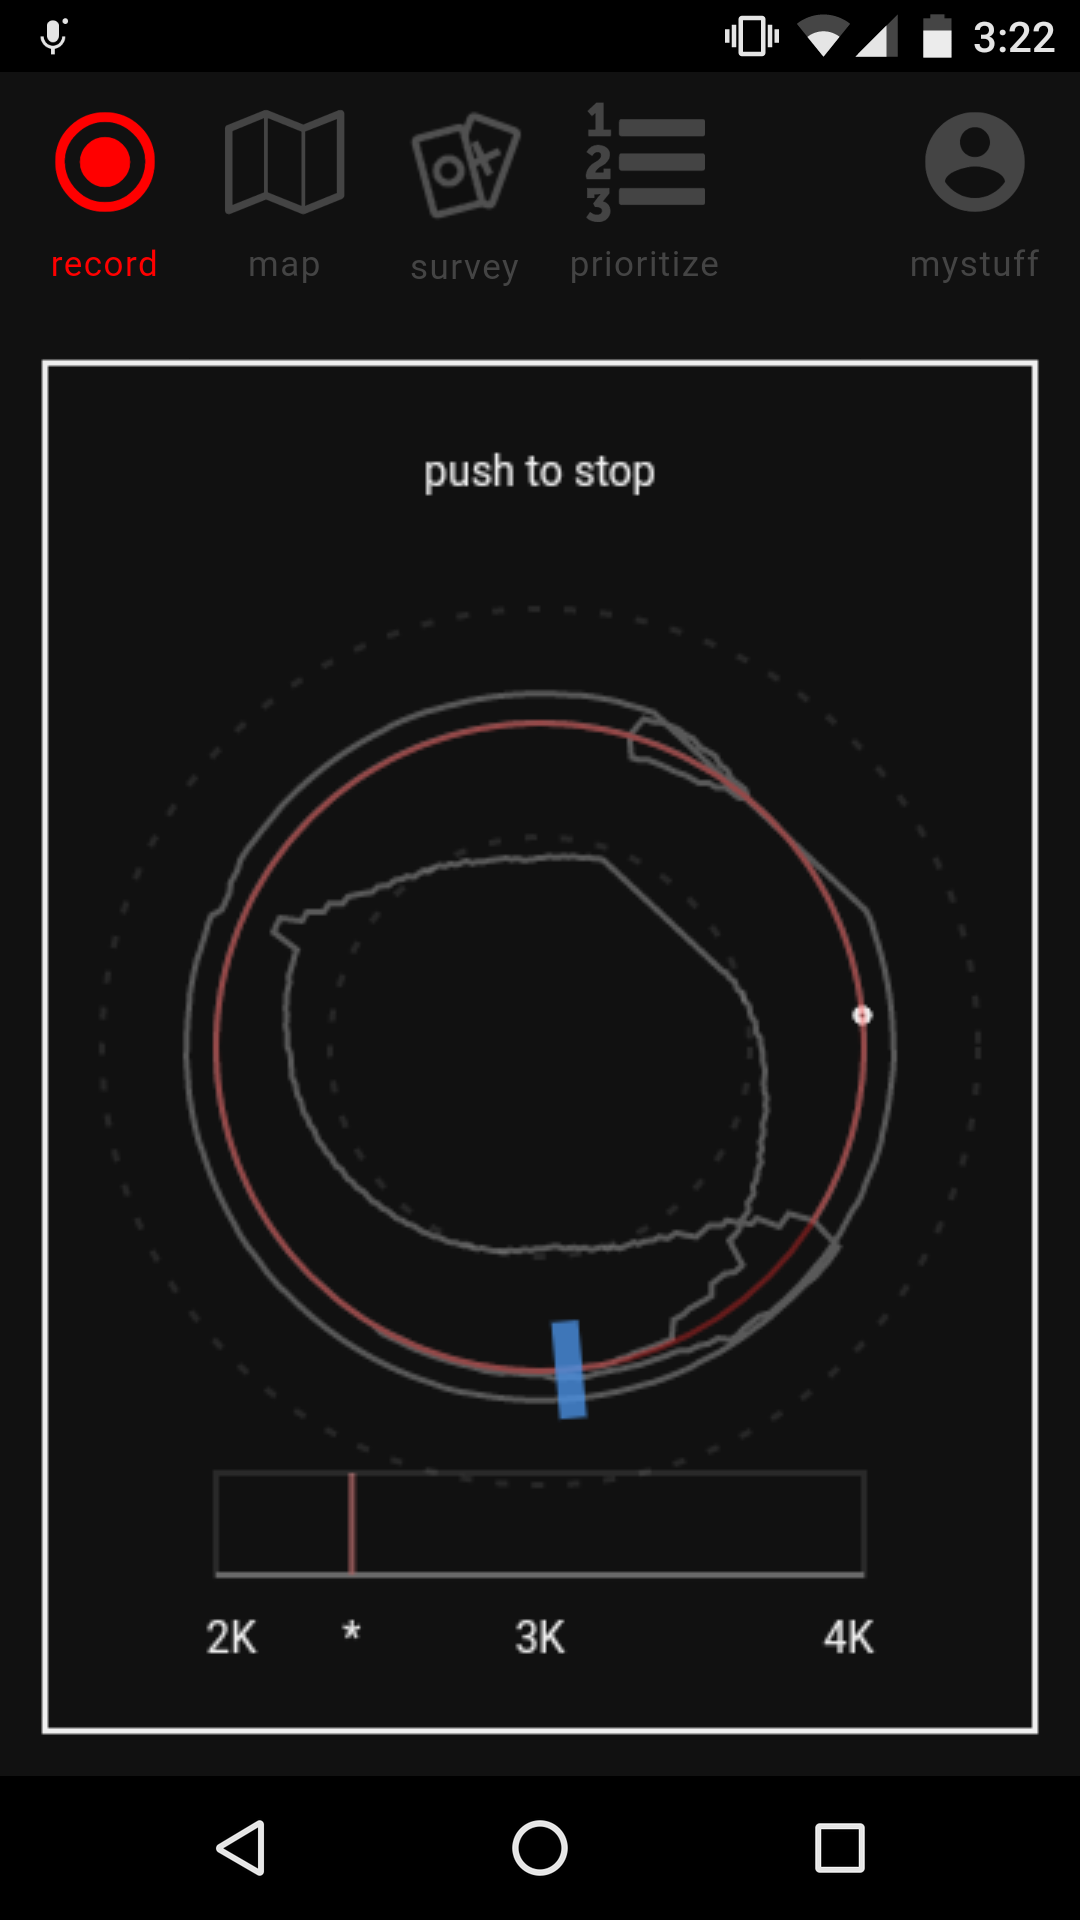
\includegraphics[width=0.6\textwidth]{chapters/4/fig/interface_recording.png}
  \caption[interface: Record]{recording view}
  \label{fig:interface_record}
\end{figure}

Figure\ref{fig:interface_record} is the main view when users ride their bike and
record the events. The primary function is to detect the user's bike's ring
and send it to the server. Based on given data from the calibration, the
application looks into the target frequency and validates two thresholds;
the slope through the adjacent frequency values and the duration that slop
threshold persisted (time limit).
Refer to\ref{appendix:time} for details on the method of ring bell detection.
The initial detection will store two things in memory; 1. The latest
geolocation and 2. A sound of 4 seconds before the detection.
\footnote{the recorder holds a data array with constant length and stores
  each sound input, overwrites the data each time it is full. This data array
  will be developed when saving as an audio clip. To exclude the first part
  of the detection, the system will record from -5 seconds to -1 seconds
relative to the detection.}
If once detected and  detected more than once in the succeeding 4 seconds,
the place is judged to be ``good,'' and if it is never detected, it is
judged to be ``bad.'' After the four seconds, the app will submit the
geolocation of the first location, sound data and ``good''/``bad'' label to the server, and returns to the initial state.
The users will be notified about this one ring is ``bad'' and twice means
``bad'' protocol before hand.

The interface uses animation frame to show the detection and the label data
``good'' or ``bad,'' with a circle orbiting the 4-second detection interval.
For safety reasons, when recording, other buttons are disabled to prevent
user input. Also while recording, the app will periodically query the
geolocation and store ``bread crumbs'' of geolocation.

\subsection{Map View}

\begin{figure}[htb]
  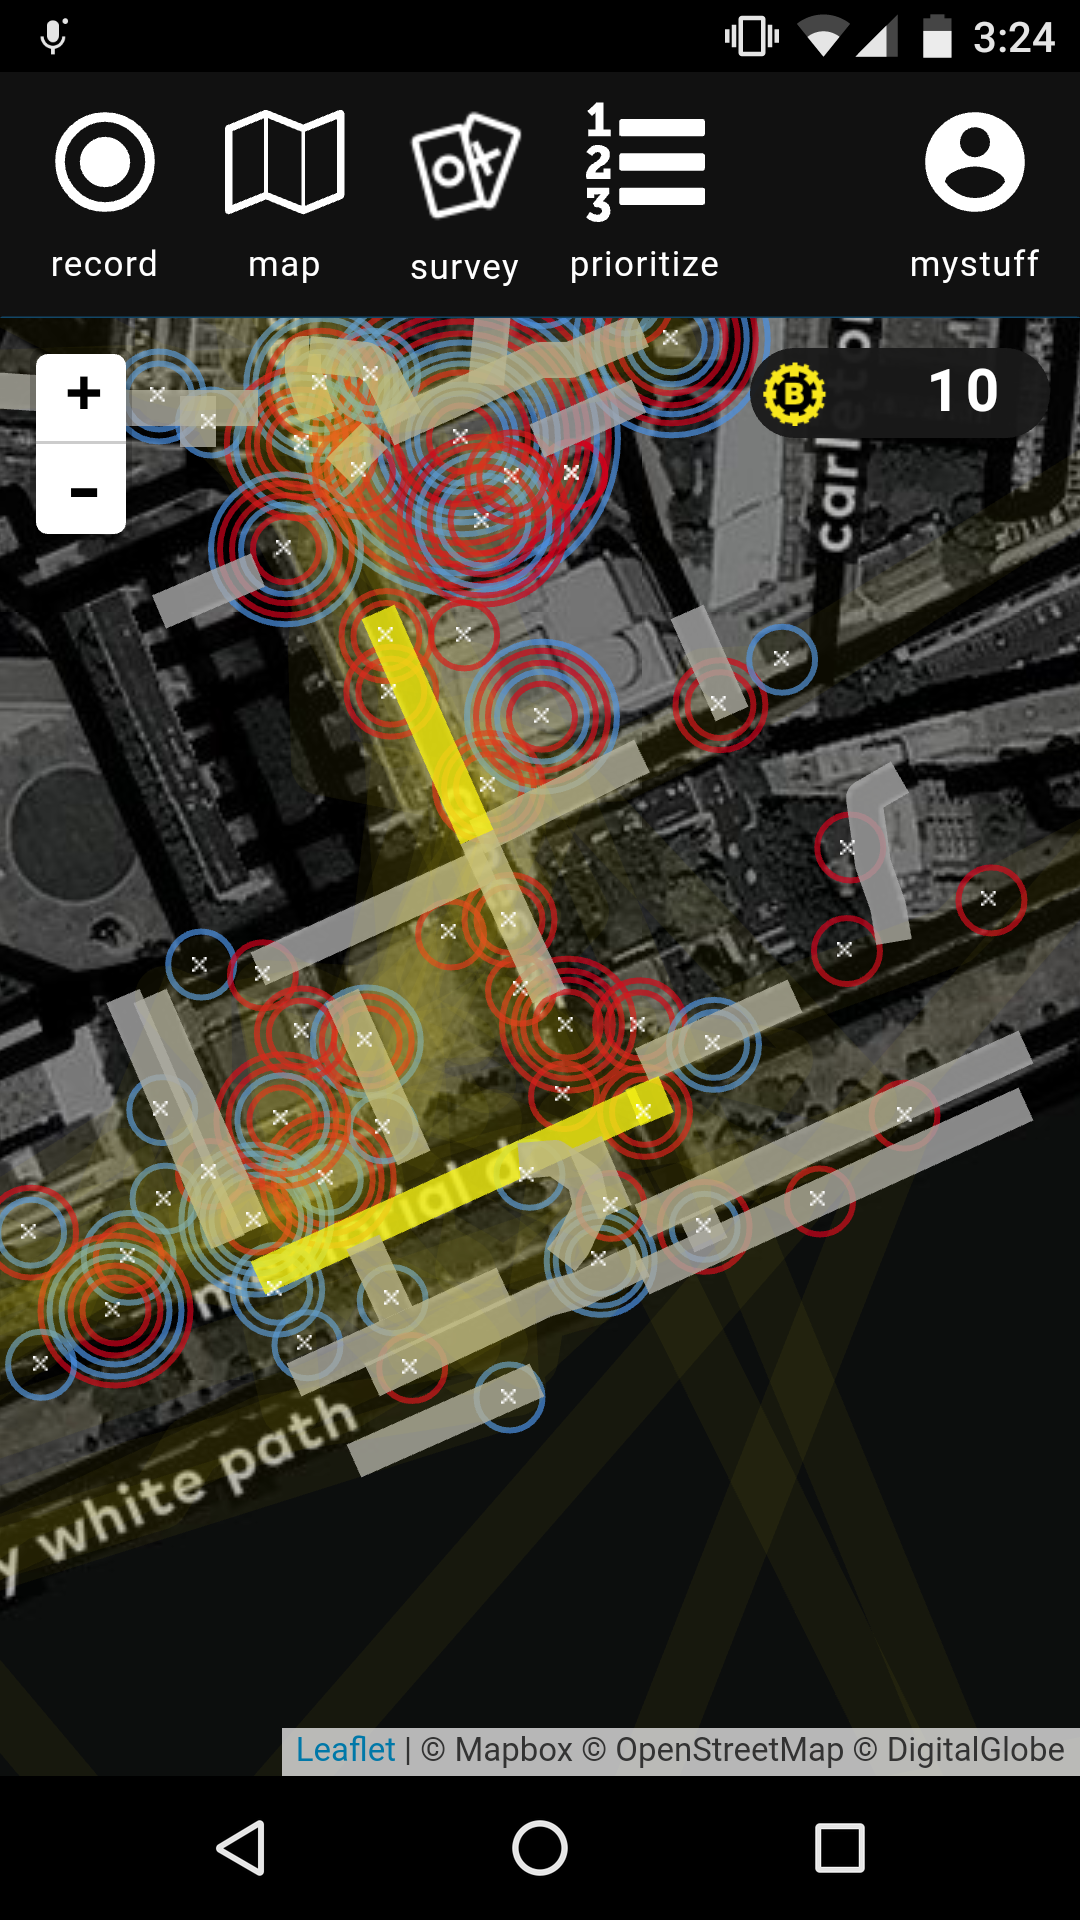
\includegraphics[width=0.6\textwidth]{chapters/4/fig/interface_map.png}               
  \caption[interface: Map]{Map view}
  \label{fig:interface_map}
\end{figure}

\begin{marginfigure}[{0cm}]
  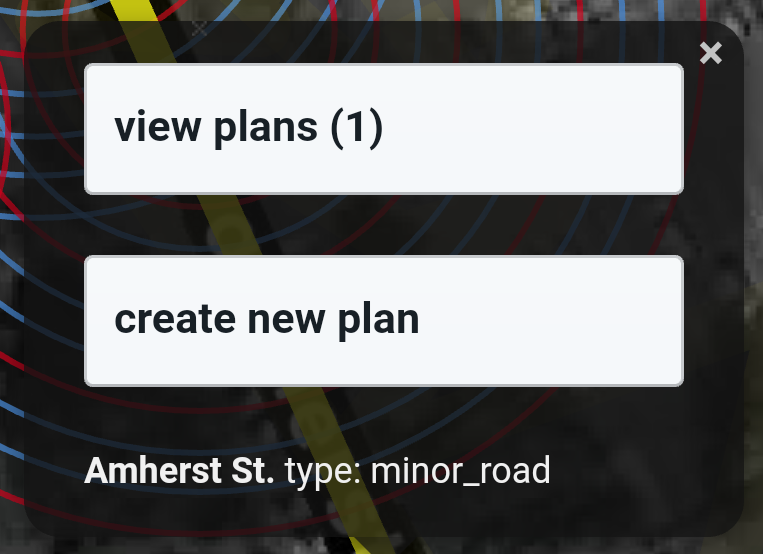
\includegraphics{chapters/4/fig/interface_popup.png}               
  \caption[interface: Popup]{a pop-up navigator linked to creating or
  voting to IMPROVEMENT PLANS}
  \label{fig:interface_popup}
\end{marginfigure}

The Map view (Figure \ref{fig:interface_map}) visualizes the data obtained by users.
The visualization includes geolocation data of people's DINGs, highlighted
roads that had one or more closest dings. The commute paths that people
took. Yellow road segments indicate that there was at least one improvement
plan submitted by any user. The roads have pop-ups (Figure\ref{fig:interface_popup}) that link to options to
existing improvement plans or the improvement creation view.




% The application was implemented as a smartphone interface
% Detecting locations that are unsafe
% detecting ring bells
% FFT performed by the microphone
% Attempt to catch specific frequency preconfigured by the setting.
% [image: bell]
% [image: interface]
% Query current condition to identify bike lane security
% Ask (mostly) binary questions to set the current
% Two reasons to ask
% have fine grain information on current situation
% ask users for current
% [image: interface]
% Visualise acquired report data
% mapping of unsafe areas
% [image: map plot]
% Solution Picking
% Solicit solutions by selecting from possible diagrammatic solutions
% Prioritisation

\subsection{Survey View}

\begin{figure}[htb]
  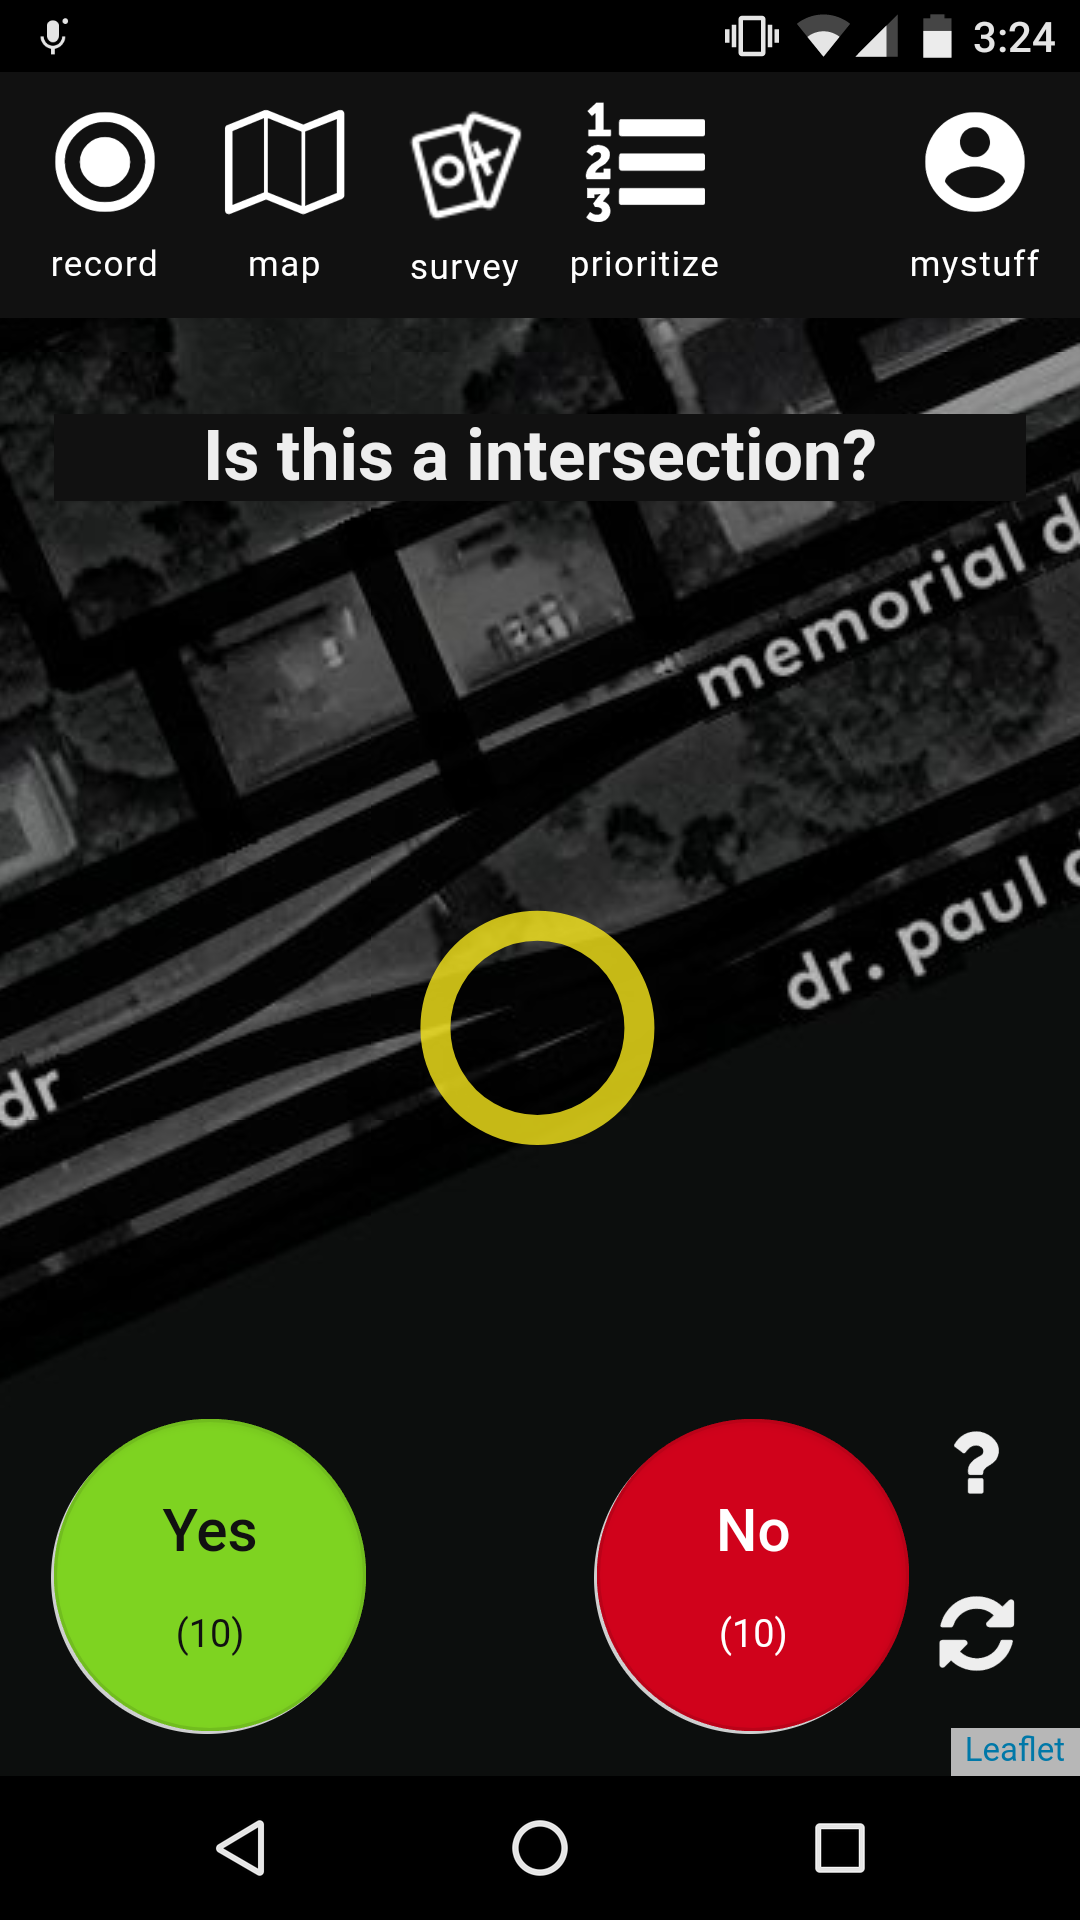
\includegraphics[width=0.6\textwidth]{chapters/4/fig/interface_survey.png}               
  \caption[interface: Survey]{Survey view}
  \label{fig:interface_survey}
\end{figure}

The survey view asks the users follow up questions to complement their ding
reporting. There are two purposes for having this feature, thus two kinds
of questions. The first purpose is to collect information that does not
exist in the Map Data such as OpenStreetMap (OSM). OSM data does not
include information about specific conditions about the bike lane, for
example, painted in green, or separated with plastic bollards.
\footnote{some Path network includes information on the existence of a bike
  lane or an attribute indicating it is a cycle path yet the data have no
guarantee that it is updated timely.} 
The type of questions that serve this purpose is for retrieving information
on the current condition. For the experiment, these questions were:

\begin{enumerate}
  \item Is this place an intersection?
  \item Was there a separated bike lane?
\end{enumerate}

Secondly, the reason for the ``Good'' / ``Bad'' judgments varies,
so requires more information to ask for specific questions why the
report occurred.
One ``Bad'' DING may mean bad because of a pothole or a car blocking the
bike lane (occasional conditions) or no bike lane (planning conditions)

\begin{enumerate}
  \item The road was bumpy.
  \item It had lots of three shades.
\end{enumerate}

\subsection{Create Improvement View}

The create improvement enables users to submit improvements to the system
to be voted by other users.
The pop-up menu that each road shows (Figure \ref{fig:interface_popup})
provide links to this view (Figure \ref{fig:interface_improvment}).
To create an IMPROVEMENT PLAN, it is required to select the SOLUTION, and if
applicable, which range to apply for the selected road. While editing, the
total BIKE COIN changes that needed for community approval. The user who
proposes any plan will need to decide the tradeoff between different
solutions and ranges.

\begin{figure}[!htb]
  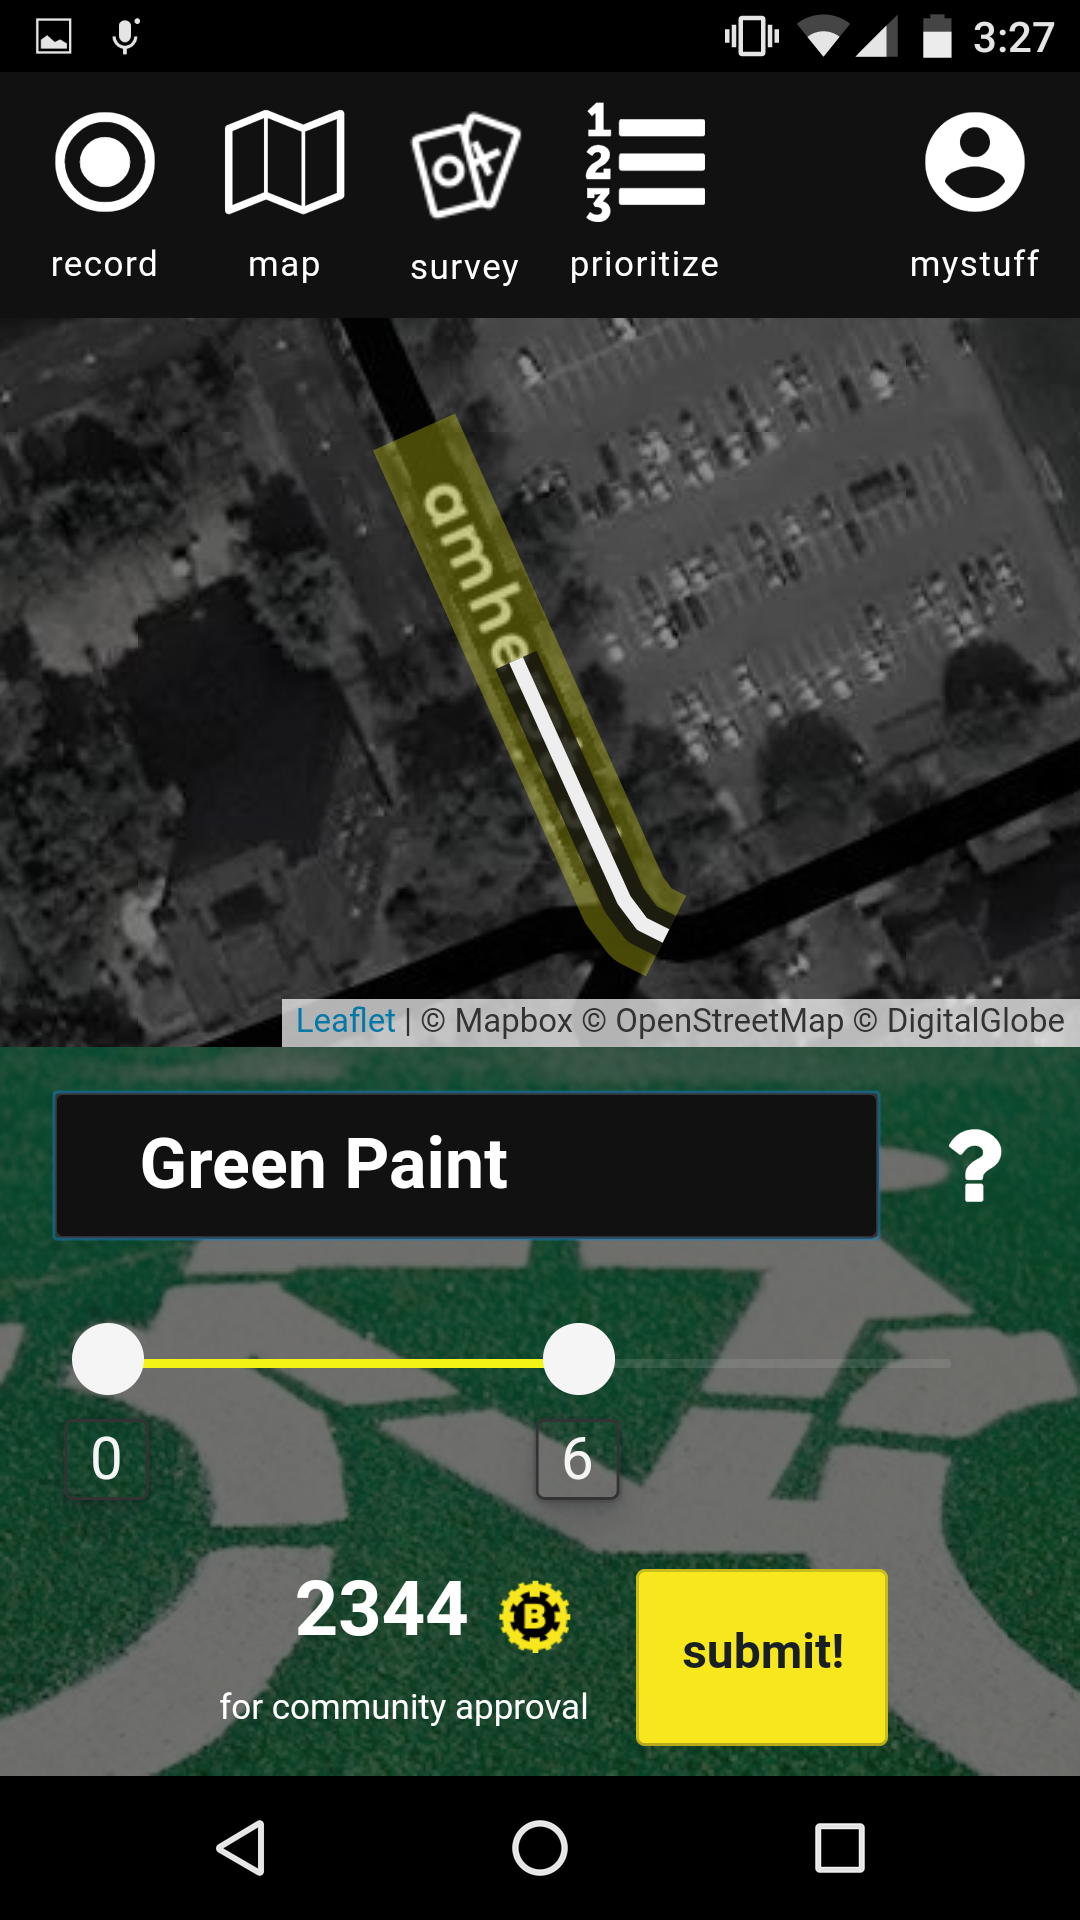
\includegraphics[width=0.6\textwidth]{chapters/4/fig/interface_solution2.png}               
  \caption[interface: Survey]{Survey view}
  \label{fig:interface_improvment}
\end{figure}

\subsection{Vote View}

Each IMPROVEMENT PLAN will have a VOTE view. It provides the interface to
distribute points for the segment. It is a four choice question, with the
option to give 0, 10, 20, and 50 BIKE COINS to the target plan. The app
permits the user to vote for their IMPROVEMENT PLANS created by themselves.

\begin{marginfigure}
  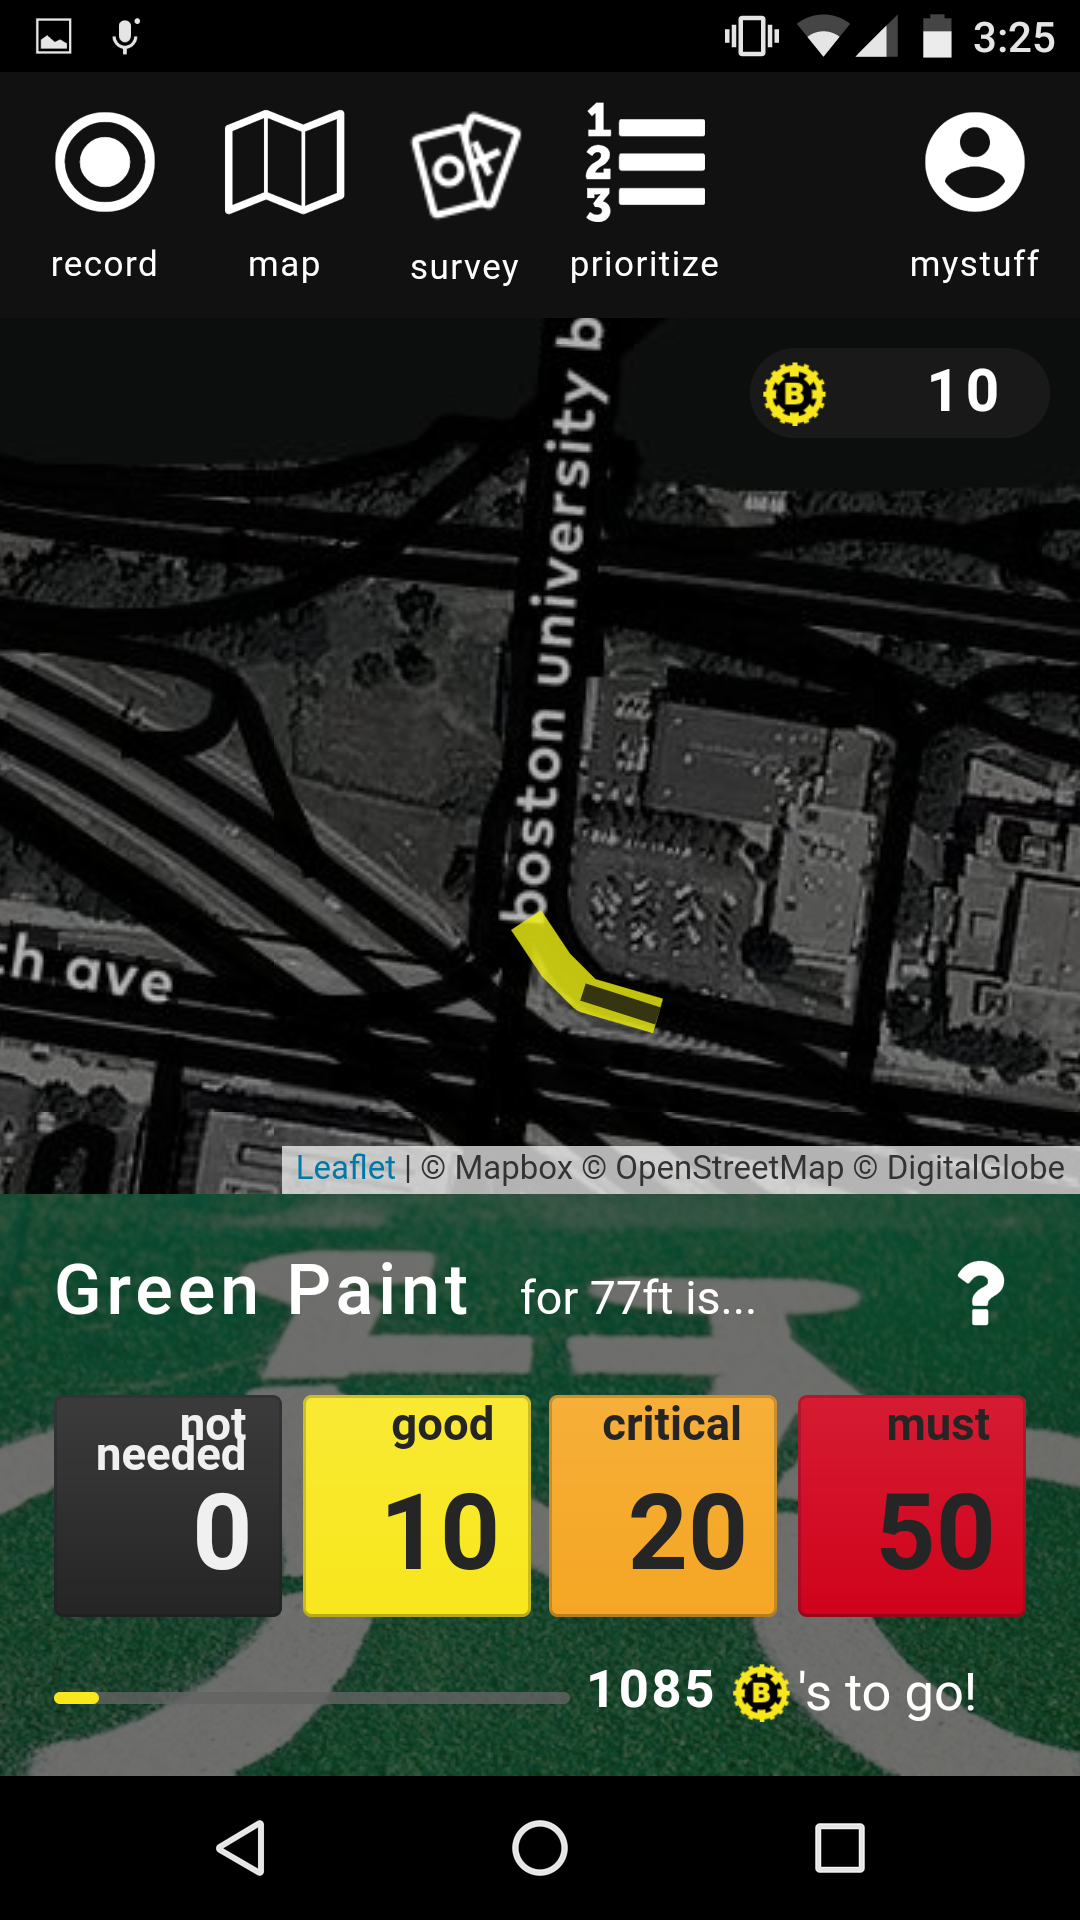
\includegraphics[width=0.6\textwidth]{chapters/4/fig/interface_vote.png}               
  \caption[interface: Vote]{Vote view}
  \label{fig:interface_vote}
\end{marginfigure}

\subsection{Improvement List View}

\begin{figure}[!htb]
  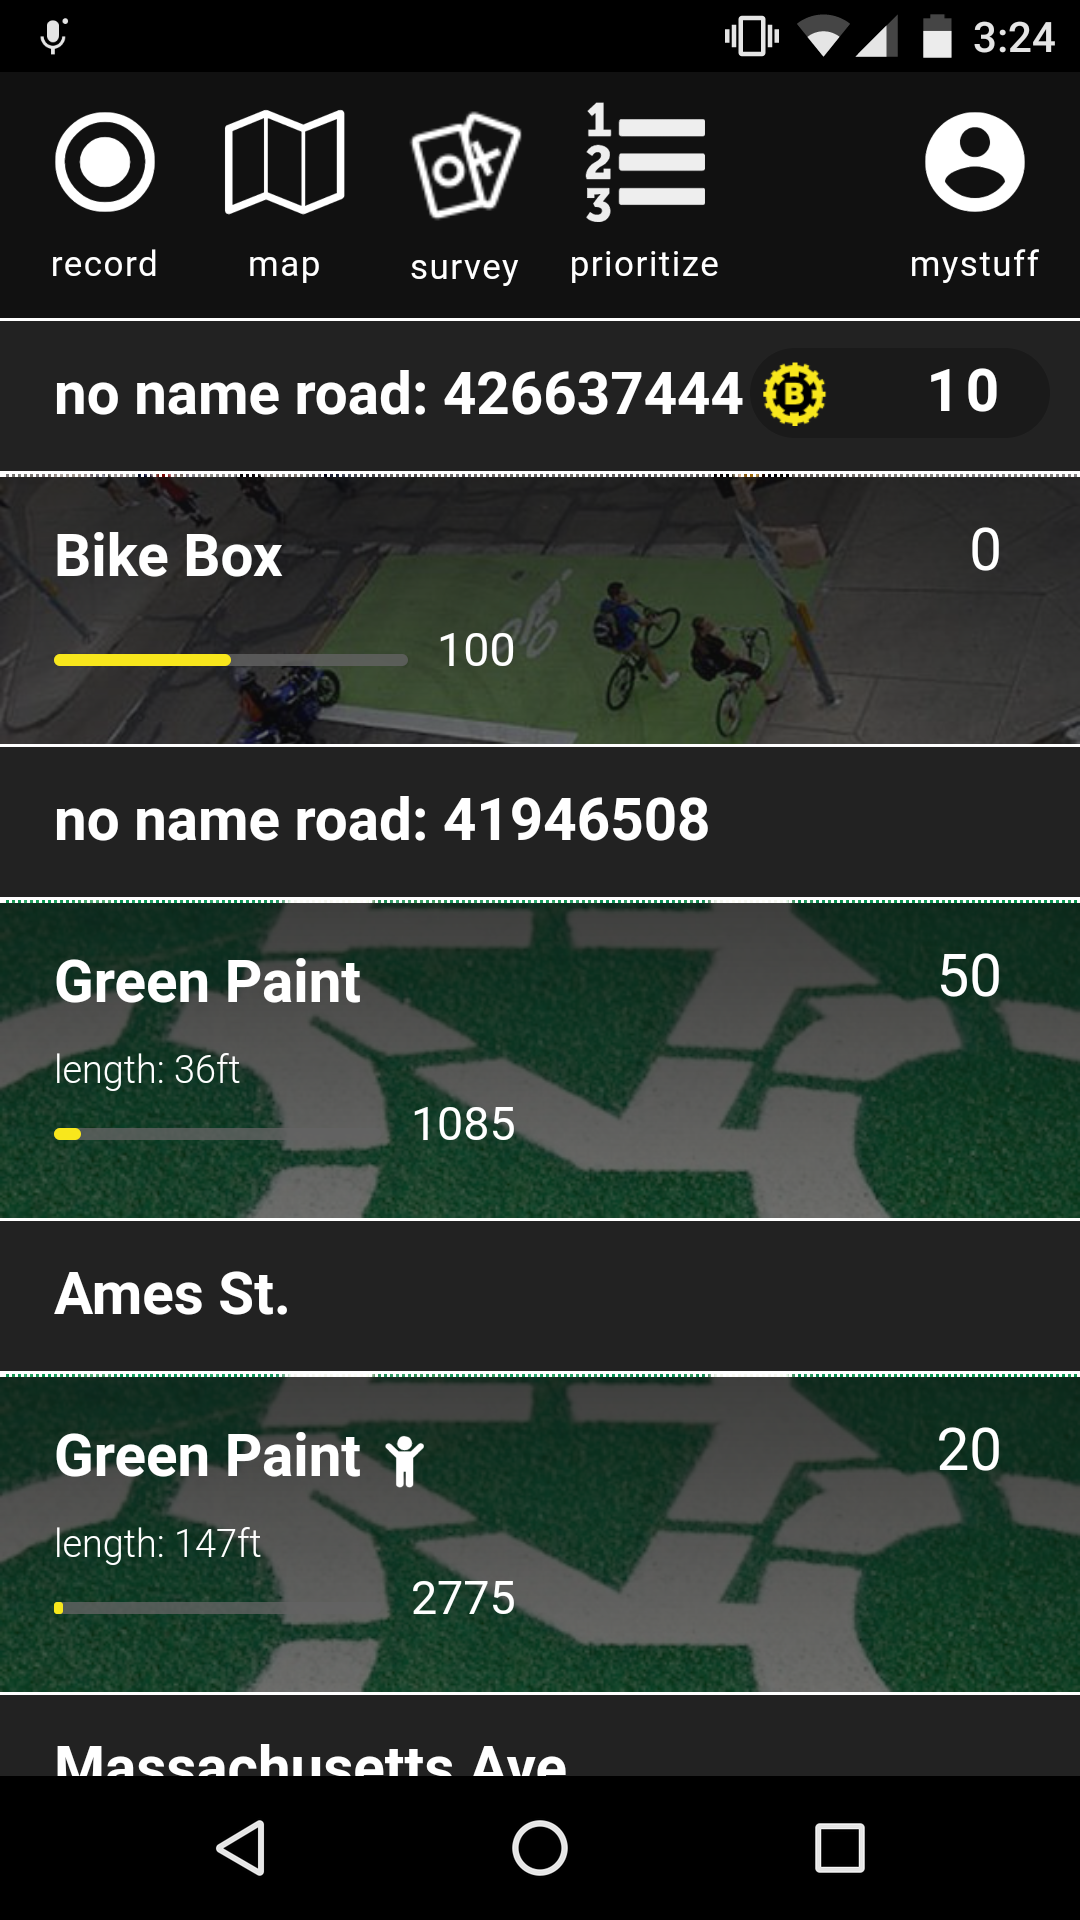
\includegraphics[width=0.6\textwidth]{chapters/4/fig/interface_list.png}               
  \caption[interface: Improvement list]{Improvement list}
  \label{fig:interface_list}
\end{figure}

The Improvement list is the where users can see a sorted list of each
improvement.
This list is sorted by the total number of BIKE COINS.

\section{Experiment Setting}

A human subject test was conducted to examine the functionality
and effectiveness of the prototype. Refer to Appendix \ref{app:COUHES} for
the complete consent form.

A total of 20 people had been recruited by email and social media posts;
the users demographic was students and individuals from local bike advocacy
groups. Out of the 20 participants, five were female subjects. Each test
had one participant.

Three participated using a bike sharing service\footnote{Hubway
\url{https://www.thehubway.com/}} others used their bike. 12 people used
the bell provided, and none owned a smartphone mount. The experiment was
conducted during the day, without rain, time slots were 9:30, 12:00, 14:00,
15:00.

Each test took around 1.5 hours. The experiment had four steps. The first
was the orientation, where the examiner introduces the objective of the
user test, gains subject's consent, asks for the initial survey, shows how
the application works, and talk about the route of the on bike experiment.

The second step is to have the users ride the bike, with the app running.
Figure \ref{fig: route} is the path that was asked for subjects to take.

\begin{figure}[!htb]
  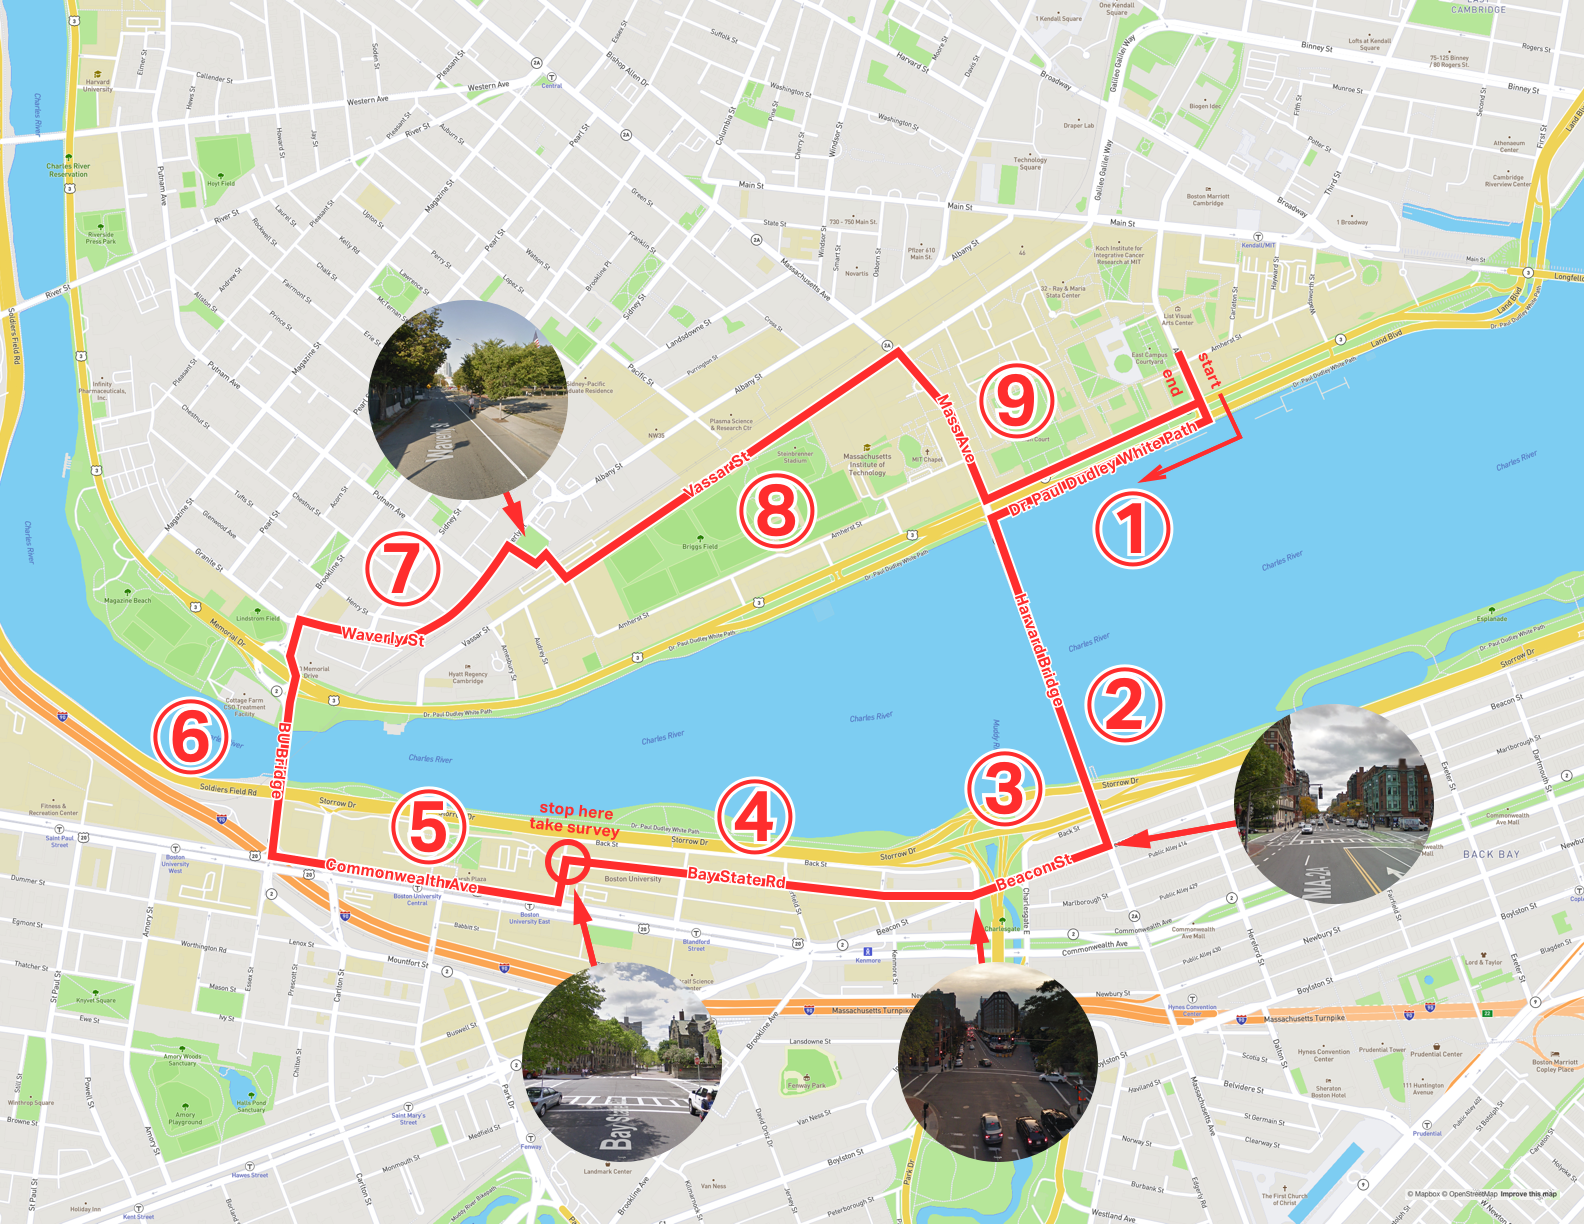
\includegraphics[width=\textwidth]{chapters/4/fig/fixed_route.png}               
  \caption[on-bike fixed route]{on-bike fixed route}
  \label{fig:route}
\end{figure}

The start location was the entrance of MIT Media Lab heading towards the
Charles river turning right taking the Dr. Paul Dudley White Path. This
path was renewed in 2017, with a bi-directional cycle path which is rare in
Cambridge. The route makes a left turn to take the Harvard Bridge, which
does not have a dedicated bike lane. Car traffic is relatively high since
there is no light until the end of the bridge. The intersection of Havard
Bridge and Beacon Street is infamous having accidents and considered one of
the most dangerous crossings. 
\footnote{a cyclist died hit by a tractor trailer in 2015
\url{https://www.bostonglobe.com/metro/2015/08/07/woman-bicyclist-injured-apparent-collision-with-vehicle-back-bay/zsjWYLZIZ324kSkmbjOaWM/story.html}}
In response to the number of accidents, the city of Boston has had modified
the lane structure for the crossing and Beacon Street. Proceeding to Beacon
Street, the route takes a slight right for Bay State Road. Park Driveway
crosses Beacon Street close to this intersection, which is also close to
the intersection of a major cross down Parkway, Storrow Drive. Bay State
Road is a one-way road with less traffic but no bike lanes and an arch of
tall trees in both sides. The users are asked to take a survey using the
app at the intersection of Back Street. Taking a short left turn, it is
Common wealth Avenue which a wide multi lane road that is a part of an
arterial route. Despite the wide road and fast traffic, there is no
separated bike lane. Subjects take the BU Bridge heading back to Cambridge.
Over the weeks of experiments, this BU Bridge was shut down to cars
allowing only pedestrians and bikers to cross.
\footnote{Boston Globe reported the happy comments from the cyclists, right
  after the shutdown. \url{https://www.bostonglobe.com/metro/2017/07/28/for-cyclists-bridge-closure-like-heaven/bBWnlm00ROV7LfZW0w7f2O/story.html}}
The BU Bridge ends with a roundabout that does not have lights or separated
bike lanes. The route turns left after the roundabout to Waverly Street,
thin single lane street. The path turns right before the park to take
Vassar Street. Vassar Street has a dedicated bikeway at the same level of
the side walk. The route returns to the Mass Avenue crossing MIT's main
entrance. This part is often crowded with tourist buses with many
pedestrians crossing. It is also close to the bridge, which the drivers
rush to catch the light with high speed. Lastly, the route heads back to
the origin using the same path, but the different side.
There is a lengthy discussion on bikes riding on sidewalks, and the law is
different depending on the area. Massachusetts law permits bikers to use
the side walks if the local city permits to do so. 
\footnote{Massachusets General Laws PartI Title XIV Chapter 85 Section 11 B
\url{https://malegislature.gov/Laws/GeneralLaws/PartI/TitleXIV/Chapter85/Section11B}}
The city of Cambridge does not ban bicycles to use the side walks in
Memorial Drive. /footnote{Sidewalk Bicycling Banned Areas.
\url{http://www.cambridgema.gov/CDD/Transportation/gettingaroundcambridge/bybike/rulesoftheroad.aspx}}

This on-bike test was designed to take approximately 30 minutes. Within the
experiment, users were required to stop and take an in-experiment survey.

After the user had come back from the trial, a discussion was held to know
how people perceived the ride with this app.

% 
% summary of results, raw data will be attached to the Appendix
% mapping
% inputs from users
% technical results
% ring detection success rate
\section{Results}
\subsection{Quatative}
% have basic statistics of the amount of data collected through the experiment
\textbf{Accident report comparison}
70/% of the bike accident reports were included in at least one ``Bad'' DING.\footnote{a DING that the have larger amount of ``Bad'' reports}
% have basic statistics of the amount of data collected through the experiment
\textbf{Ambient sound noise and `bad' report correlation}
Sound clip data did not show (Yet!), ambient noise influences
    peoples perception of ``Good'' / ``Bad'' when biking.
\tectbf{BU Bridge before and after}
The tendency of the report changed radically after the bridge shut down.

\subsection{Quantative}
A summary of the replies for the after bike discussion follows the next section will discuss the subject's response in detail:
\begin{itemize}
\item None of the people knew the standard process to change a road. 
\item Most of the people recognized that this could be useful to learn the collective opinion and maybe able to replace the current system without modification.
\item People said, ``Bad'' reports were often a moment or a point, where ``Good'' reports were often a continuous feeling.
  \item The majority of subject felt awkward when ringing the bell when there was someone in front.
\item Participants understood there are two distinct processes, and felt it is useful to have them integrated into one.
\item The interview has a section that discusses the two usages of the app. One is open access where the citizen can download and use when ever they wish, create improvement plans and vote for them without any limitation. The second possibility is the city concentrating to a specific road they think they need to improve and set predefined improvement plans 

    than being told by the city to concentrate on a particular route.
\end{itemize}

\section{Evaluation}
\subsection{Analytical side}
\begin{itemize}
  \item Most of the people said the app functioned as intended, while there
    were some complaints it was unstable when large vehicles (trucks and buses) passed.
  \item The analytical side showed that this method might be an indicator
    of accidents, yet it is important to know where people moved, since the
    data may be biased towards particular routes.
  \item It is hard and too early to say that both DING positions and sound
    clip data are a good predictor of bike accidents.
  \item Relativeness - There were multiple times people stated that they
    felt danger when the bike lane disappeared. Talking that safeness is
    relative to the previous feeling of being safe. This comment is an
    indication that already it is a wicked problem.
\end{itemize}

\subsection{Synthetic side}
\item It was rather obvious that none of the people knew how to propose an
  improvement plan. The trend was the same for the foreigner's regarding
  their own country.
\item Most people said there is no disadvantage having a proposal layer on
  top of the data layer. Some stated it is better to have the analytical
  side and synthetic side integrated since it is easy to go back and forth.
  While there were some opinions that the integration could be much more
  intuitive.
\item There are two ways to use this app in practice. A controlled
  engagement where the city provides the particular segment and for  the
  call for data collection and improvement plans. In contrast, a free
  platform that the citizens/participants are free to collect data and
  submit improvement plans to their demand. Most of the participants
  preferred the free version, yet lead to a dilemma that if it was free to
  use, there is very few chance to encounter that app or ever installing it
  and may be used and dominated by serious bikers, which is exclusive and
  opposite having a grassroots method.

